\documentclass[11pt]{article}

\usepackage[utf8]{inputenc}
\usepackage[T1]{fontenc}
\usepackage[margin=1in]{geometry}
\usepackage{amsmath,amssymb,amsthm}
\usepackage{booktabs}
\usepackage{graphicx}
\usepackage{xcolor}
\usepackage{tikz}
\usetikzlibrary{arrows.meta,positioning,calc,shapes.geometric,fit,backgrounds}
\usepackage[font=small,labelfont=bf]{caption}
\usepackage{hyperref}
\usepackage{natbib}
\hypersetup{colorlinks=true,linkcolor=blue!50!black,citecolor=blue!50!black,urlcolor=blue!50!black}

\newcommand{\code}[1]{\texttt{#1}}
\newcommand{\R}{\mathbb{R}}
\DeclareMathOperator{\LN}{LN}
\DeclareMathOperator{\MHA}{MHA}
\DeclareMathOperator{\GELU}{GELU}
\DeclareMathOperator{\softmax}{softmax}
\DeclareMathOperator{\clip}{clip}
\DeclareMathOperator{\sg}{sg}

\title{The Minute Forecaster (TradingGame v4):\\
       a Supervised Transformer for the Next-Minute Return Distribution}
\author{Prabal Negi \\ \small \texttt{market-agent} project \\[2pt]
        \small Architecture and evaluation write-up drafted with Claude (Anthropic)}
\date{October 2026}

\begin{document}
\maketitle

\begin{abstract}
\noindent
Version 4 of \texttt{TradingGame} drops the reinforcement-learning game and learns the market's short-term
dynamics directly. A single transformer, shared by every stock, reads the last $M{=}96$ one-minute states of
$N$ stocks and predicts, at every minute and for every stock, a \emph{distribution} for the next minute's
log-return (a Student-$t$ with a location and a bounded scale), together with the next timestamp. One-minute
returns are nearly unpredictable in the mean, so the scale of the distribution is where most of the learnable
signal is. This note specifies the data pipeline, every layer with its matrix form and parameter count, the
loss ($\beta$-weighted negative log-likelihood), the training procedure, and the evaluation protocol, including
a linear autoregressive baseline scored by exactly the same code. In one 80-epoch run (59{,}749 parameters, 80
training and 80 disjoint validation companies, validated on 2025) the network improves the validation likelihood
over a constant per-stock scale by $0.140$ nats per target and over an EWMA scale by $0.160$, reaches a mean-forecast skill
of $8.6\%$ over predicting zero, and keeps its 68\% and 95\% intervals calibrated; the autoregressive baseline gets
$0.050$ nats and $1.6\%$ skill.
\end{abstract}

\tableofcontents

% ─────────────────────────────────────────────────────────────────────────
\section{Problem and scope}

The v1--v3 game trains a policy by reinforcement learning on 15-minute or hourly bars; after a full v3
run the policy had not learned anything useful. v4 steps back from decisions and asks a prior question:
\emph{how much of the market's next minute can be predicted at all?} It strips the input to stock prices
(no news, macro series or portfolio state) and makes the task supervised.

\paragraph{Task.} For a window of $M$ consecutive trading minutes of $N$ stocks, predict for every stock $i$ and every
minute $t$ of the window the distribution of the next minute's return $r_{t+1,i}$, and the description of the next
bar's timestamp. The forecast at minute $t$ may use minutes $\le t$ only (causality).

\paragraph{Design decisions.}
\begin{itemize}
  \item \emph{A distribution, not a point.} A one-minute return is dominated by noise, so a point forecast is almost
        always close to zero. The model outputs a location $\mu$ and a scale $\sigma$ and is trained by likelihood.
  \item \emph{Shared weights.} No parameter depends on which company a column holds, so the training and validation
        companies may differ and so may $N$.
  \item \emph{Forecaster first.} A trading policy on top of the forecaster is a later step; this note covers the forecaster only.
\end{itemize}

% ─────────────────────────────────────────────────────────────────────────
\section{Data}\label{sec:data}

\subsection{The minute cache}

\code{build\_minute\_cache.jl} reads each symbol's 1-minute OHLCV file and aligns all symbols on one axis of
trading days $\times$ 375 session minutes (09:15--15:29). A day joins the axis when at least 20\% of the
symbols have 10 or more session bars in it. A minute with no row keeps the previous close (forward fill) and is flagged
\emph{untraded}; a row with volume above zero is \emph{traded}. Only returns and the traded flag are stored; the
model never sees a price level. The percent log-return of the close is
\begin{equation}
  r_{t,i} \;=\; \clip\!\Big(100\ln\frac{c_{t,i}}{c_{t-1,i}},\ \pm 10\Big),
\end{equation}
and before it enters the network it is divided by $s$, the root-mean-square return of the traded minutes of the cache
($s\approx 0.32$ for the cache used in Section~\ref{sec:results}). All distributional quantities below are therefore in units of one typical
move, which makes the output scale bounds and the Student-$t$ comparable across caches.

\subsection{Time features and the timestamp description}

For the bar at minute $t$ the model receives $K{=}5$ time features
\begin{equation}
  \tau_t = \Big[\tfrac{m_t}{375},\ \sin\tfrac{2\pi w_t}{5},\ \cos\tfrac{2\pi w_t}{5},\ \ln(1+g_t),\ \mathbf 1[\text{first bar of the day}]\Big]^{\top}\in\R^{5},
\end{equation}
with $m_t$ the minute of the day, $w_t\in\{0,\dots,4\}$ the weekday and $g_t$ the number of calendar days since the
previous bar. The three-number \emph{timestamp description} the model predicts for the next bar is $\big(m_{t+1}/375,\ \ln(1+g_{t+1}),\ w_{t+1}/4\big)$.

\subsection{Per-stock context}

A stock has no fixed slot in the input, so it is described to the network by two numbers computed from the 375
bars (one trading day) \emph{before} the window starts: the mean absolute return and the traded fraction,
\begin{equation}
  c_i=\Big[\tfrac1{375}\sum_{t=s-375}^{s-1}|r_{t,i}|,\ \ \tfrac1{375}\sum_{t=s-375}^{s-1}\mathbf 1[\text{traded}_{t,i}]\Big]^{\top},
\end{equation}
for a window starting at bar $s$. No token therefore sees a bar later than its own minute.

\subsection{Windows, targets and masks}

A training example is a window of $M{=}96$ consecutive bars. Every position $t$ of the window yields a target for
every stock, $y_{t,i}=r_{t+1,i}/s$, so one window gives $M\times N$ targets (teacher forcing; the causal mask keeps them
honest). A target counts, $m_{t+1,i}=1$, only if the stock \emph{traded} in minute $t{+}1$ and minute $t{+}1$ is not the first
bar of a day. A forward-filled zero is not information, and the overnight gap is not a one-minute move.

\subsection{Train and validation split}\label{sec:split}

Validation differs from training in \emph{both} companies and dates: the training companies and the validation companies are
disjoint lists, and every window lies entirely inside its date range (in the run reported here, training
2022-01-03 to 2024-12-30 and validation 2025-01-01 to 2025-12-30). No target is shared between the two. Because
market-wide movements are shared across stocks, a validation score on unseen companies but training dates could be flattered by
the market itself, so the evaluation reports three sets (Section~\ref{sec:eval}).

% ─────────────────────────────────────────────────────────────────────────
\section{Architecture}\label{sec:arch}

\begin{table}[h]
\centering
\caption{Notation. Default values are those of the run in Section~\ref{sec:results}.}
\begin{tabular}{@{}llr@{}}
\toprule
Symbol & Meaning & Value \\
\midrule
$N$ & stocks in a window (any number) & 80 \\
$M$ & minutes in a window & 96 \\
$d,\ H,\ d_h=d/H$ & model width, heads, head size & 32, 4, 8 \\
$L$ & causal time blocks & 4 \\
$K$ & time features per minute & 5 \\
$F=1+K+2$ & input features per stock token & 8 \\
$\nu$ & Student-$t$ degrees of freedom & 4 \\
\bottomrule
\end{tabular}
\end{table}

\begin{figure}[t]
\centering
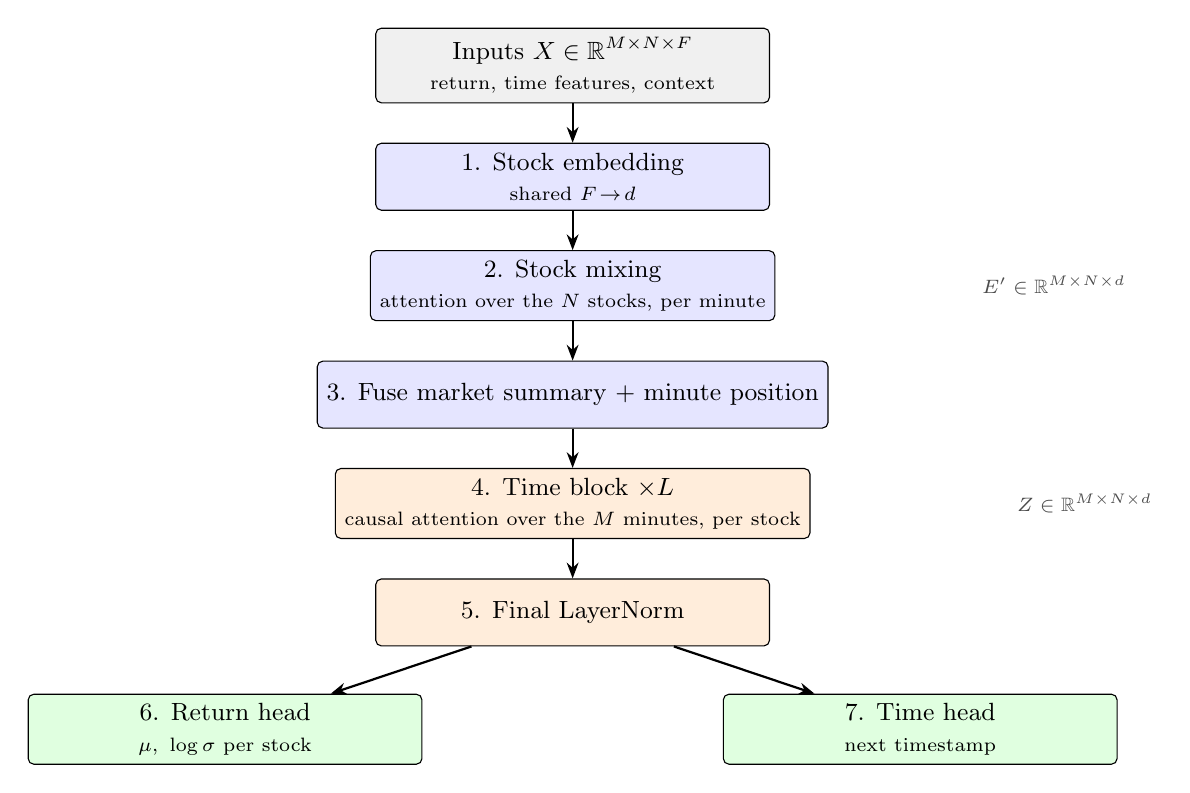
\begin{tikzpicture}[
  node distance=5mm and 6mm,
  box/.style={draw, rounded corners=2pt, minimum height=8.5mm, minimum width=50mm, align=center, font=\small},
  stk/.style={box, fill=blue!10},
  tim/.style={box, fill=orange!14},
  hd/.style={box, fill=green!12},
  inp/.style={box, fill=gray!12},
  arr/.style={-{Stealth[length=2mm]}, thick},
  lab/.style={font=\scriptsize\itshape, text=black!70}]
  \node[inp] (in) {Inputs $X\in\R^{M\times N\times F}$\\{\scriptsize return, time features, context}};
  \node[stk, below=of in] (emb) {1. Stock embedding\\{\scriptsize shared $F\!\to\! d$}};
  \node[stk, below=of emb] (mix) {2. Stock mixing\\{\scriptsize attention over the $N$ stocks, per minute}};
  \node[stk, below=of mix] (fus) {3. Fuse market summary + minute position};
  \node[tim, below=of fus] (blk) {4. Time block $\times L$\\{\scriptsize causal attention over the $M$ minutes, per stock}};
  \node[tim, below=of blk] (fin) {5. Final LayerNorm};
  \node[hd, below left=6mm and -6mm of fin] (ret) {6. Return head\\{\scriptsize $\mu,\ \log\sigma$ per stock}};
  \node[hd, below right=6mm and -6mm of fin] (tm) {7. Time head\\{\scriptsize next timestamp}};
  \draw[arr] (in)--(emb); \draw[arr] (emb)--(mix); \draw[arr] (mix)--(fus); \draw[arr] (fus)--(blk); \draw[arr] (blk)--(fin);
  \draw[arr] (fin)--(ret); \draw[arr] (fin)--(tm);
  \node[lab, right=3mm of mix, xshift=22mm] {$E'\in\R^{M\times N\times d}$};
  \node[lab, right=3mm of blk, xshift=22mm] {$Z\in\R^{M\times N\times d}$};
\end{tikzpicture}
\caption{Data flow for one window. Blue layers mix information \emph{across stocks} within one minute; orange layers attend \emph{along time} within one stock.}
\label{fig:flow}
\end{figure}

The network (Figure~\ref{fig:flow}) has two attention axes on the $M\times N\times d$ tensor. Stock mixing lets a stock's
token use what the rest of the market did in the same minute; the time blocks let it use its own history. Normalisation is
pre-norm \citep{xiong2020prenorm} with LayerNorm \citep{ba2016layernorm}, and the feed-forward network uses the GELU
\citep{hendrycks2016gelu}. Attention follows \citet{vaswani2017attention}.

\subsection{Building blocks}

For $A\in\R^{n\times d}$ ($n$ tokens, one per row), with $\mu=\tfrac1d A\mathbf 1_d$ and $\sigma^2=\tfrac1d(A-\mu\mathbf 1^{\top})^{\odot 2}\mathbf 1_d$,
\begin{align}
  \LN(A) &= \big(A-\mu\mathbf 1_d^{\top}\big)\oslash\sqrt{\sigma^2\mathbf 1_d^{\top}+\varepsilon}\ \odot\ \mathbf 1\gamma^{\top}+\mathbf 1\beta^{\top},\\
  Q&=AW_Q^{\top}+\mathbf 1b_Q^{\top},\quad K=AW_K^{\top}+\mathbf 1b_K^{\top},\quad V=AW_V^{\top}+\mathbf 1b_V^{\top},\\
  O_h&=\softmax\!\Big(\tfrac{Q_hK_h^{\top}}{\sqrt{d_h}}+B\Big)V_h,\quad h=1,\dots,H,\\
  \MHA(A)&=\big[O_1\ \cdots\ O_H\big]W_O^{\top}+\mathbf 1b_O^{\top},\\
  \GELU(x)&=\tfrac12 x\Big(1+\tanh\!\big(\sqrt{2/\pi}\,(x+0.044715\,x^3)\big)\Big),
\end{align}
where $Q_h,K_h,V_h\in\R^{n\times d_h}$ are the $h$-th column blocks, $W_Q,W_K,W_V,W_O\in\R^{d\times d}$, and $B$ is an additive mask
($B=0$ for stock mixing, lower-triangular $0/-\infty$ for the time blocks).

\subsection{Layers}

\paragraph{1. Stock embedding.} For minute $t$ the token matrix is $X_t=[\,r_t\ \ \mathbf 1_N\tau_t^{\top}\ \ C\,]\in\R^{N\times F}$ and
\begin{equation}
  E_t = X_tW_e^{\top}+\mathbf 1_Nb_e^{\top}\in\R^{N\times d},\qquad t=1,\dots,M,
\end{equation}
with $W_e\in\R^{d\times F}$ shared by every stock and every minute.

\paragraph{2. Stock mixing.} Within each minute the $N$ tokens attend to each other with no positional code, so the order of the stocks is irrelevant:
\begin{equation}
  E'_t=E_t+\MHA\big(\LN(E_t)\big),\qquad s_t=\tfrac1N E_t'^{\top}\mathbf 1_N\in\R^{d}.
\end{equation}
The mean $s_t$ is the market summary of the minute; $S=[s_1\ \cdots\ s_M]^{\top}\in\R^{M\times d}$.

\paragraph{3. Fuse and position.} For each stock $i$ (with $E'_{\cdot,i}\in\R^{M\times d}$ its tokens over time),
\begin{equation}
  Z_i=E'_{\cdot,i}+SW_s^{\top}+\mathbf 1_Mb_s^{\top}+P\in\R^{M\times d},\qquad W_s\in\R^{d\times d},\ P\in\R^{M\times d}\text{ learned}.
\end{equation}

\paragraph{4. Time blocks ($L$ of them).} For one stock, the $M$ tokens are a sequence and minute $t$ may only look at minutes $s\le t$:
$B_{ts}=0$ for $s\le t$ and $-\infty$ otherwise. Each block is
\begin{align}
  Z&\leftarrow Z+\MHA\big(\LN(Z)\big),\\
  Z&\leftarrow Z+\Big(\GELU\big(\LN(Z)W_1^{\top}+\mathbf 1b_1^{\top}\big)\Big)W_2^{\top}+\mathbf 1b_2^{\top},
\end{align}
with $W_1\in\R^{4d\times d}$ and $W_2\in\R^{d\times 4d}$; every block has its own weights, and the $N$ sequences share them.

\paragraph{5. Final LayerNorm.} $H=\LN(Z)\in\R^{M\times d}$ per stock, $H\in\R^{M\times N\times d}$ overall.

\paragraph{6. Return head.} One linear map shared by every stock turns each token into a location and a raw scale:
\begin{equation}
  \begin{pmatrix}\mu_{t,i}\\ q_{t,i}\end{pmatrix}=W_rh_{t,i}+b_r,\qquad
  \log\sigma_{t,i}=c+a\tanh q_{t,i},\qquad r_{t+1,i}/s\ \sim\ t_\nu\big(\mu_{t,i},\sigma_{t,i}\big),
\end{equation}
with $W_r\in\R^{2\times d}$, $c=-0.5$ and $a=2.5$, which keeps $\sigma$ between about $0.05$ and $7$ return units.

\paragraph{7. Time head.} Averaging the tokens of all stocks at a minute, $\bar h_t=\tfrac1N\sum_iH_{t,i}$,
\begin{equation}
  \hat\tau_{t+1}=\pi(\tau_t)+D\big(W_\tau\bar h_t+b_\tau\big)\in\R^{3},\qquad D=\operatorname{diag}\big(\tfrac1{375},1,1\big),
\end{equation}
where $\pi(\tau_t)$ is the calendar's own guess (not learned): one session minute on within a day, and at the last minute of the day the next weekday
(with a gap of one day, three after a Friday). Only holidays defeat this rule, so the head learns a small correction and the minute is exact by construction.
$W_\tau$ and $b_\tau$ are initialised at zero.

\subsection{Parameters and cost}

Counting weights and biases (LayerNorm has $2d$, the multi-head attention $4(d^2+d)$), the parameters are
\begin{equation}
  \underbrace{Fd+d}_{\text{embed}}+\underbrace{2d+4(d^2+d)}_{\text{mixing}}+\underbrace{d^2+d+Md}_{\text{fuse}}
  +L\underbrace{\big(4d+4(d^2+d)+8d^2+5d\big)}_{\text{time block}}+\underbrace{2d}_{\text{final LN}}+\underbrace{2d+2}_{\text{return}}+\underbrace{3d+3}_{\text{time}}.
\end{equation}
For $M{=}96$, $L{=}4$, $F{=}8$ this gives 59{,}749 parameters at $d{=}32$, 228{,}037 at $d{=}64$ and 890{,}245 at $d{=}128$
(matching the code's count for each). The width $d$ is a hyperparameter to sweep and keep the smallest that matches the best validation result.

The cost is dominated by the attention scores: stock mixing computes $M\cdot H\cdot N^2$ entries and each time block $N\cdot H\cdot M^2$. On a 16\,GB card a batch of 32 windows of 80 stocks fits; a batch of
128 does not.

% ─────────────────────────────────────────────────────────────────────────
\section{Output distribution and loss}\label{sec:loss}

\subsection{\texorpdfstring{Student-$t$}{Student-t} likelihood}

With the location $\mu$ and scale $\sigma$ above, the per-target negative log-likelihood of $y$ under a Student-$t$ with $\nu$ degrees of freedom is
\begin{equation}
  \ell_\nu(y;\mu,\sigma)=\log\sigma+\tfrac{\nu+1}{2}\log\!\Big(1+\tfrac1\nu\big(\tfrac{y-\mu}{\sigma}\big)^2\Big)+c_\nu,\qquad
  c_\nu=\log\Gamma\!\big(\tfrac\nu2\big)-\log\Gamma\!\big(\tfrac{\nu+1}2\big)+\tfrac12\log(\nu\pi).
\end{equation}
Its standard deviation is $\sigma\sqrt{\nu/(\nu-2)}$, so $\nu>2$ is required; the default is $\nu=4$. Minute returns have heavy tails: under a Gaussian, one extreme minute
produces a huge gradient and a few outliers can dominate training, whereas the Student-$t$ loss grows only logarithmically in the error. The Gaussian ($\ell(y;\mu,\sigma)=\log\sigma+\tfrac12(\tfrac{y-\mu}{\sigma})^2+\tfrac12\log 2\pi$) and the
Huber loss \citep{huber1964robust} on the location alone (quadratic below one return unit, linear above; no scale, so no uncertainty) are selectable alternatives.

\subsection{\texorpdfstring{$\beta$}{Beta}-weighted likelihood}

Fitting a location and a scale jointly has a known failure: a model can lower the likelihood by inflating $\sigma$ where its mean fits badly, so the mean stops improving. Following
\citet{seitzer2022pitfalls}, each term is weighted by $\sigma^{2\beta}$ \emph{held constant} (stop-gradient),
\begin{equation}
  \mathcal L_{\text{ret}}=\frac{\sum_{t,i}m_{t+1,i}\,\sg\!\big(\sigma_{t,i}^{2\beta}\big)\,\ell_\nu\!\big(y_{t,i};\mu_{t,i},\sigma_{t,i}\big)}{\sum_{t,i}m_{t+1,i}},\qquad\beta=0.5,
\end{equation}
where $\beta=0$ is the plain likelihood. Because the weight changes as $\sigma$ moves, the \emph{training loss is not comparable across epochs}; evaluation always reports the unweighted likelihood.

\subsection{Total loss}

The timestamp term is the mean squared error of the description (the minute fraction measured in minutes),
$\mathcal L_\tau=\tfrac1M\sum_t\|\hat\tau_{t+1}-\tau_{t+1}\|^2$, and
\begin{equation}
  \mathcal L=\mathcal L_{\text{ret}}+\lambda_\tau\mathcal L_\tau,\qquad\lambda_\tau=0.1.
\end{equation}

% ─────────────────────────────────────────────────────────────────────────
\section{Training}

\begin{itemize}
  \item \textbf{Batches.} Random window starts into the cache (no file reads in the loop). An ``epoch'' is a fixed number of such batches (500 steps), not a pass over the data, because windows overlap.
  \item \textbf{Optimiser.} AdamW \citep{loshchilov2019adamw} with peak learning rate $3\times10^{-4}$, weight decay $0.01$, a linear warm-up over 200 steps, then a cosine decay to a tenth of the peak
        \citep{loshchilov2017sgdr}, and gradient-norm clipping at 1.0. Dropout is 0.1.
  \item \textbf{Checkpoint.} After each epoch the three evaluation sets are scored and the checkpoint with the lowest validation negative log-likelihood is kept.
  \item \textbf{Number types.} The forward and backward pass run in \code{float32} (default), \code{float16} or \code{float64}. \code{float16} keeps float32 master weights, scales the loss dynamically
        \citep{micikevicius2018mixed} (a step whose gradients overflow is skipped and counted), and computes the loss in float32; the checkpoint is always float32. Float8 has no usable Julia type and is not supported.
  \item \textbf{Implementation.} Julia with Flux \citep{innes2018flux}; the run's configuration is one TOML file read by \code{scripts/train\_minute\_forecaster.jl}, and the training page streams its progress.
\end{itemize}

% ─────────────────────────────────────────────────────────────────────────
\section{Evaluation}\label{sec:eval}

Because one-minute returns are close to unpredictable in the mean, every score is reported next to trivial predictors, on the same masked targets.

\paragraph{Evaluation sets.} \code{val} (validation companies, validation dates; decides the checkpoint), \code{val\_train\_\allowbreak companies} (training companies, validation dates) and \code{train} (training companies, training dates).
Comparing \code{val} to \code{val\_train\_\allowbreak companies} isolates the cost of new companies; comparing \code{val\_train\_\allowbreak companies} to \code{train} isolates the cost of new dates.

\paragraph{Location.} With $\mu$ the predicted location and $y$ the target,
\begin{equation}
  \text{skill}=1-\frac{\operatorname{MSE}(\mu,y)}{\operatorname{MSE}(0,y)},\qquad
  \text{hit rate}=\Pr\big[\operatorname{sign}\mu=\operatorname{sign}y\ \big|\ y\neq0,\ m=1\big].
\end{equation}
Skill $0$ means no better than predicting no move, and negative means worse; $50\%$ is a coin for the hit rate. The \emph{repeat-last} baseline sets $\mu_{t,i}=r_{t,i}$.

\paragraph{Scale and calibration.} The likelihood is scored against two baselines that predict a zero location,
\begin{equation}
  \text{gain}_{\text{const}}=\overline{\ell_\nu(y;0,\sigma_{\text{const}})}-\overline{\ell_\nu(y;\mu,\sigma)},\qquad
  \text{gain}_{\text{EWMA}}=\overline{\ell_\nu(y;0,\sigma_{\text{EWMA}})}-\overline{\ell_\nu(y;\mu,\sigma)},
\end{equation}
in nats per target, where $\sigma_{\text{const}}$ is one scale per stock (its RMS return, converted to the distribution's scale) and $\sigma_{\text{EWMA}}$ is the exponentially weighted average of recent squared returns with decay $0.94$ per minute
\citep{riskmetrics1996}. Both baseline scales are clamped to the range the model's own $\sigma$ can take, so a stock that never moves cannot win by a scale of zero. A positive gain means the predicted scale carries information beyond the baseline.
\emph{Coverage} is the fraction of targets inside the model's own central 68\% and 95\% interval, $|y-\mu|/\sigma\le h_p$ with $h_p$ the Student-$t$ quantile; a calibrated model scores about $0.68$ and $0.95$ (the likelihood is a strictly proper scoring rule
\citep{gneiting2007scoring}, so it rewards calibration and sharpness together).
The report also gives the skill per 15-minute slot of the session and per stock, and the predicted against the realised standard deviation per slot (the predicted value is $\sigma\sqrt{\nu/(\nu-2)}$; heavy tails put the realised RMS above it).

\paragraph{Timestamp.} Accuracy of the minute, day-gap and weekday predictions within a small tolerance. It is close to 100\% by construction (Section~\ref{sec:arch}) and shows the head works, not that the market is predictable.

\subsection{A linear autoregressive baseline}

To see how much of the result lagged returns alone give, \code{scripts/ar\_baseline.jl} fits a linear model on the same windows and scores it with the same code.
The location is a ridge regression of the next return on the last $k{=}10$ returns of the same stock, with one set of coefficients shared by all stocks (lags before the window start are zero, as the network also sees nothing before its window).
For the scale, each stock has a level $m_i$, its mean absolute return over the previous day divided by its traded fraction; the ratio $E|y-\mu|/m_i$ is regressed on the 25 minute-of-day buckets of the session, the $k$ latest $|r|/m_i$ and an exponentially weighted $|r|/m_i$, and the prediction is multiplied by $m_i$ and divided by
$c(\nu)=E|t_\nu|$ to obtain $\sigma$ (for $\nu=4$, $c=1$). The model is multiplicative across stocks because volatility is. It has no cross-stock term and no non-linearity.

% ─────────────────────────────────────────────────────────────────────────
\section{Results of one run}\label{sec:results}

\paragraph{Setup.} $d=32$ (59{,}749 parameters), $M=96$, $L=4$, $H=4$, batch 32, 80 epochs of 500 steps, float32, $\nu=4$, $\beta=0.5$, on an RTX 5060\,Ti (0.75\,s per step, 8.3\,hours). 80 training companies (2022-01-03 to 2024-12-30) and 80 disjoint validation companies (2025), 256 evaluation windows per set.
All numbers are from the saved checkpoint of the last epoch (the validation likelihood had plateaued: it improved by $0.0001$ from epoch 70 to 80).

\begin{table}[h]
\centering\footnotesize\setlength{\tabcolsep}{4pt}
\caption{Network and linear baseline on the three evaluation sets. NLL is in nats per target, in return-scale units, so only the gains are comparable across caches.}
\begin{tabular}{@{}llrrrrrr@{}}
\toprule
Set & Model & NLL & gain const $\sigma$ & gain EWMA $\sigma$ & skill & hit rate & 95\% cov. \\
\midrule
\code{val}                 & AR(10)      & 0.7205 & 0.050 & 0.071 & 1.6\%  & 55.4\% & 93.6\% \\
                           & transformer & 0.6309 & 0.140 & 0.160 & 8.6\%  & 60.3\% & 95.6\% \\
\addlinespace
\code{val\_train\_companies} & AR(10)    & 0.9529 & 0.038 & 0.085 & 2.3\%  & 53.7\% & 91.7\% \\
                           & transformer & 0.8467 & 0.145 & 0.191 & 10.2\% & 59.8\% & 95.3\% \\
\addlinespace
\code{train}               & AR(10)      & 1.0483 & 0.064 & 0.092 & 3.2\%  & 54.6\% & 92.0\% \\
                           & transformer & 0.9450 & 0.167 & 0.196 & 11.6\% & 59.9\% & 95.2\% \\
\bottomrule
\end{tabular}
\end{table}

\paragraph{Reading the table.}
\begin{itemize}
  \item \emph{Scale is the main result.} The network beats a constant per-stock scale by $0.140$ nats and an EWMA scale by $0.160$ on unseen companies and dates; the linear scale model gets about a third of that.
  \item \emph{The mean is weak but real.} Skill is $8.6\%$ on validation (the repeat-last baseline is strongly negative: bid--ask bounce makes a minute partly reverse the previous one). The linear model's skill is $1.6\%$ and its location coefficients are the bounce: $-0.21$ on the latest return, decaying to about $-0.02$ by lag 10.
        Adding lags does not help (30 or 90 lags give the same skill and a worse scale gain).
  \item \emph{Calibration.} The network's 68\% and 95\% intervals contain $67.6\%$ and $95.6\%$ of validation targets; the linear model's 95\% interval is too narrow ($93.6\%$).
  \item \emph{Generalisation.} The gap between the training and validation companies on the validation dates is $1.6$ skill points and between training and validation dates $1.4$ more, so the network is not badly over-fitted.
  \item \emph{Spread.} On validation only 1 of 71 scored stocks has negative skill (the worst $-3.3\%$, the best about $16\%$; nine stocks traded too rarely to score); by time of day the skill stays between about $6\%$ and $11\%$, highest in the first 15 minutes.
\end{itemize}

% ─────────────────────────────────────────────────────────────────────────
\section{Limitations and next steps}

\begin{itemize}
  \item \textbf{Is it tradeable?} The best per-stock skill is on thinly traded names, where bid--ask bounce and stale quotes are likely the source. A skill that exists only at quoted prices that cannot be traded is not a trading edge; the next test is to check the traded fraction against the per-stock skill and then to simulate execution costs.
  \item \textbf{One run, one seed.} Differences below about $0.2$ skill points between epochs or runs are within the noise of 256 windows per set. The width sweep ($d\in\{32,64,128\}$, same seed) has not been repeated on the final cache.
  \item \textbf{The baseline is not the strongest linear model.} It uses only a stock's own lags. A baseline with cross-stock or market-wide terms would score higher, so the network's margin is an upper bound on what cross-stock and non-linear structure add.
  \item \textbf{Stock-specific biases shared by both.} The constant-scale baseline uses each stock's RMS measured on the evaluation targets themselves, which is slightly favourable to the baselines; it applies equally to the network and the linear model.
  \item \textbf{Absolute numbers depend on the cache.} The return scale $s$ and the set of days and symbols changed between caches, so likelihood and skill from different caches are not comparable.
  \item \textbf{No decisions yet.} A policy on top of the forecaster (position sizing from $\mu$ and $\sigma$, costs, risk limits) is a separate, later step.
\end{itemize}

\bibliographystyle{plainnat}
\bibliography{forecaster_v4}

\end{document}
